% Báo cáo đồ án Khai thác tập phổ biến — biên dịch bằng XeLaTeX
% Bố cục theo IEEE conference format: 2 cột, 10pt, Times, lề IEEE.
\documentclass[10pt,twocolumn,letterpaper]{article}
\usepackage[top=0.75in,bottom=1in,left=0.625in,right=0.625in,columnsep=0.25in]{geometry}
\usepackage{fontspec}
\setmainfont{TeX Gyre Termes}
\usepackage{amsmath,amssymb}
\usepackage{graphicx,booktabs,multirow,array}
\usepackage[font=footnotesize,labelsep=period]{caption}
\usepackage{enumitem}
\usepackage{titlesec}
\usepackage[hidelinks]{hyperref}
\usepackage{cite}
\usepackage{algorithm}
\usepackage{algpseudocode}
\usepackage{listings}
\usepackage{xcolor}
\lstset{basicstyle=\ttfamily\scriptsize,columns=fullflexible,keepspaces=true,frame=single,
  rulecolor=\color{black!30},xleftmargin=2pt,xrightmargin=2pt,breaklines=true,
  keywordstyle=\bfseries,morekeywords={function,for,end,if,in,return,continue,while,break},
  commentstyle=\itshape\color{black!60},morecomment=[l]{\#}}
\floatname{algorithm}{Thuật toán}
\renewcommand{\algorithmicrequire}{\textbf{Vào:}}
\renewcommand{\algorithmicensure}{\textbf{Ra:}}
\setlist{nosep,leftmargin=*}
\setlength{\parindent}{1em}

% Tiêu đề mục kiểu IEEE: I. TIÊU ĐỀ (chữ hoa nhỏ, căn giữa); A. Mục con (nghiêng)
\renewcommand\thesection{\Roman{section}}
\renewcommand\thesubsection{\Alph{subsection}}
\renewcommand\thesubsubsection{\arabic{subsubsection}}
\titleformat{\section}{\centering\normalfont\scshape}{\thesection.}{0.5em}{}
\titleformat{\subsection}{\normalfont\itshape}{\thesubsection.}{0.5em}{}
\titleformat{\subsubsection}{\normalfont\itshape}{\thesubsubsection)}{0.5em}{}
\titlespacing*{\section}{0pt}{8pt}{4pt}
\titlespacing*{\subsection}{0pt}{6pt}{3pt}
\titlespacing*{\subsubsection}{0pt}{4pt}{2pt}
\renewcommand{\figurename}{Hình}
\renewcommand{\tablename}{Bảng}
\renewcommand{\refname}{Tài liệu tham khảo}
\renewcommand{\thetable}{\Roman{table}}
\renewcommand{\sup}{\operatorname{sup}}
\newcommand{\D}{\mathcal{D}}

\begin{document}
\twocolumn[{%
\begin{center}
{\fontsize{22}{26}\selectfont Khai thác tập phổ biến bằng họ thuật toán Apriori:\\ cài đặt lại bằng Julia, thực nghiệm và ứng dụng\par}
\vspace{12pt}
{\normalsize
\begin{tabular}{c@{\hspace{3em}}c@{\hspace{3em}}c}
\textit{Thành viên 1} & \textit{Thành viên 2} & \textit{Thành viên 3}\\
MSSV: \texttt{xxxxxxxx} & MSSV: \texttt{xxxxxxxx} & MSSV: \texttt{xxxxxxxx}
\end{tabular}\\[4pt]
\textit{Nhóm 21 — Bộ môn Khoa học máy tính, Trường ĐH Khoa học Tự nhiên, ĐHQG-HCM}\par}
\vspace{14pt}
\end{center}}]

\noindent\textbf{\textit{Tóm tắt}—Khai thác tập phổ biến (Frequent Itemset Mining, FIM) là bước nền của bài toán luật kết hợp. Nhóm cài đặt lại từ đầu bằng Julia ba thuật toán trong bài báo gốc của Agrawal và Srikant~\cite{agrawal1994} — Apriori, AprioriTid, AprioriHybrid — cùng một biến thể tối ưu biểu diễn tidset bằng \texttt{BitVector} (đếm support bằng phép AND và popcount). Trên 4 CSDL benchmark (Chess, Mushroom, Retail, T10I4D100K) với 7 mức minsup mỗi CSDL, cả 4 biến thể cho kết quả khớp 100\% với thư viện tham chiếu SPMF ở 103/103 lần so sánh. Bản BitVector nhanh hơn bản cơ bản 18–80 lần trên dữ liệu dày và nhanh hơn SPMF tới 5 lần trên T10I4D100K ở minsup thấp, nhưng tốn bộ nhớ trên dữ liệu thưa có nhiều item. Nhóm áp dụng cài đặt vào hai bài toán thực tế: phân tích giỏ hàng trên Groceries (125 luật, top-10 theo lift chỉ ra các cụm mua sắm đồ tươi và sữa) và phân tích thành phần genome SARS-CoV-2, nơi FIM tái phát hiện hiện tượng ức chế dinucleotide CpG đã được ghi nhận trong y văn.}

\vspace{4pt}
\noindent\textbf{\textit{Từ khoá}—frequent itemset mining, Apriori, AprioriTid, luật kết hợp, Julia, bitset, SPMF.}

%======================================================================
\section{Giới thiệu}
Cho một CSDL giao dịch, bài toán \emph{khai thác tập phổ biến} (frequent itemset mining — FIM) tìm mọi tập mục (itemset) xuất hiện trong ít nhất một tỉ lệ \emph{minsup} các giao dịch. Đây là bước tốn kém nhất khi sinh luật kết hợp (association rules)~\cite{agrawal1993}, và là nền tảng của phân tích giỏ hàng (market basket analysis), phát hiện mẫu trong dữ liệu web, log hệ thống hay dữ liệu sinh học.

Nhóm chọn thuật toán \textbf{Apriori} (nhóm ``tập phổ biến cơ bản'' trong danh mục SPMF~\cite{spmf2016}) và đọc trực tiếp bài báo gốc \emph{Fast Algorithms for Mining Association Rules}~\cite{agrawal1994}. Bài báo đề xuất ba thuật toán dùng chung bước sinh ứng viên \texttt{apriori-gen} nhưng khác nhau ở cách đếm support: Apriori (quét lại CSDL mỗi mức), AprioriTid (thay CSDL bằng tập ứng viên theo từng giao dịch $\bar{C}_k$) và AprioriHybrid (chuyển từ Apriori sang AprioriTid khi $\bar{C}_k$ đủ nhỏ). Nhóm cài đặt lại cả ba, thêm một biến thể tối ưu dùng tidset dạng bit, và đóng góp:
\begin{itemize}
\item Cài đặt Julia thuần (chỉ dùng thư viện chuẩn và \texttt{DataStructures.jl}), CLI đọc/ghi định dạng SPMF, bộ unit test tự động (Mục~\ref{sec:impl}).
\item Thực nghiệm trên 4 CSDL benchmark: tính đúng đắn, thời gian, số itemset, bộ nhớ, khả năng mở rộng và ảnh hưởng của độ dài giao dịch, so sánh với SPMF (Mục~\ref{sec:exp}).
\item Hai ứng dụng thực tế chạy hoàn toàn bằng cài đặt của nhóm (Mục~\ref{sec:app}).
\end{itemize}
Mã nguồn, notebook Colab tái thực hiện mọi kết quả và dữ liệu được công bố trong repository GitHub của nhóm.

%======================================================================
\section{Các công trình liên quan}
Bài toán luật kết hợp được Agrawal, Imieliński và Swami đặt ra năm 1993 cùng thuật toán AIS~\cite{agrawal1993}, vốn sinh ứng viên ngay trong lúc quét CSDL nên tạo ra rất nhiều ứng viên không cần thiết. Apriori~\cite{agrawal1994} giải quyết vấn đề này bằng cách sinh ứng viên mức $k$ \emph{chỉ} từ $L_{k-1}$ và tỉa bằng tính chất anti-monotone; bài báo báo cáo Apriori nhanh hơn AIS và SETM từ 3 lần tới hơn một bậc độ lớn trên dữ liệu tổng hợp T$x$I$y$D$z$ — chính bộ sinh dùng để tạo T10I4D100K.

Các hướng tiếp theo chia thành ba nhóm theo cách biểu diễn dữ liệu, đúng như phân loại trong SPMF~\cite{spmf2016}. (i) \emph{Ngang, sinh ứng viên}: Apriori, AprioriTid, DHP, DIC~\cite{brin1997} — DIC đồng thời giới thiệu độ đo \emph{interest} (lift) dùng trong ứng dụng của nhóm. (ii) \emph{Dọc}: Eclat~\cite{zaki2000} lưu tidset cho mỗi itemset và tính support bằng giao tập, duyệt theo chiều sâu trong lớp tương đương tiền tố; dEclat dùng diffset để giảm bộ nhớ trên dữ liệu dày; MAFIA và Index-BitTableFI dùng bitmap. Biến thể tối ưu của nhóm mượn biểu diễn bitmap của nhóm này nhưng vẫn giữ chiến lược theo mức của Apriori. (iii) \emph{Cây mẫu, không sinh ứng viên}: FP-Growth~\cite{han2000} nén CSDL thành FP-tree và khai thác đệ quy trên các cây điều kiện, thường nhanh hơn Apriori nhiều lần trên dữ liệu dày. Các so sánh độc lập như FIMI~\cite{goethals2003} và Zheng và cộng sự~\cite{zheng2001} cho thấy không có thuật toán thắng trên mọi loại dữ liệu: hiệu năng phụ thuộc mạnh vào mật độ và phân bố độ dài giao dịch — một quan sát mà Chương~2 của báo cáo này cũng tái hiện giữa các biến thể Apriori.

Về ngôn ngữ, Julia~\cite{bezanson2017} biên dịch JIT theo kiểu của đối số (multiple dispatch), cho phép viết mã ở mức trừu tượng cao mà vẫn đạt tốc độ gần C khi các hàm ổn định kiểu; \texttt{BitVector} của thư viện chuẩn lưu 64 bit mỗi từ máy và cài đặt phép AND, đếm bit theo từ.

%======================================================================
\section{Cơ sở lý thuyết và thuật toán}\label{sec:theory}
\subsection{Định nghĩa}
Cho tập item $I=\{i_1,\dots,i_m\}$ và CSDL $\D=\{t_1,\dots,t_N\}$, mỗi giao dịch $t_j\subseteq I$. \emph{Support} của itemset $X\subseteq I$ là số giao dịch chứa $X$:
\begin{equation}
\sup(X)=\left|\{\,t\in\D : X\subseteq t\,\}\right|.
\end{equation}
Với ngưỡng tương đối $\mathit{minsup}\in(0,1]$, ngưỡng tuyệt đối là $\sigma=\lceil \mathit{minsup}\cdot N\rceil$ (giống SPMF); $X$ là \emph{tập phổ biến} nếu $\sup(X)\ge\sigma$. Gọi $L_k$ là tập các tập phổ biến kích thước $k$ và $C_k$ là tập \emph{ứng viên} kích thước $k$.

\textbf{Tính chất Apriori (anti-monotone).} Nếu $X\subseteq Y$ thì $\sup(X)\ge\sup(Y)$; do đó mọi tập con của một tập phổ biến đều phổ biến, và một ứng viên có tập con không phổ biến có thể bị loại mà không cần đếm.

\textbf{Luật kết hợp.} Với $X\cap Y=\emptyset$, luật $X\Rightarrow Y$ có
\begin{align}
\mathrm{supp}(X\Rightarrow Y)&=\sup(X\cup Y)/N,\\
\mathrm{conf}(X\Rightarrow Y)&=\sup(X\cup Y)/\sup(X),\\
\mathrm{lift}(X\Rightarrow Y)&=\mathrm{conf}(X\Rightarrow Y)\,/\,\big(\sup(Y)/N\big).
\end{align}
Lift $>1$ nghĩa là $X$ và $Y$ xuất hiện cùng nhau nhiều hơn mức kỳ vọng nếu độc lập~\cite{brin1997}.

\subsection{Sinh ứng viên \texttt{apriori-gen}}
Các itemset được lưu dưới dạng dãy item tăng dần. $C_k$ sinh từ $L_{k-1}$ qua hai bước~\cite{agrawal1994}:
\begin{itemize}
\item \textbf{Join:} ghép $p,q\in L_{k-1}$ có chung $k-2$ item đầu và $p_{k-1}<q_{k-1}$ thành $p\cup\{q_{k-1}\}$.
\item \textbf{Prune:} loại ứng viên $c$ nếu tồn tại tập con $(k-1)$ phần tử của $c$ không thuộc $L_{k-1}$.
\end{itemize}
Vì $L_{k-1}$ được sắp theo thứ tự từ điển, các itemset chung tiền tố nằm liền nhau nên vòng join có thể dừng sớm (\texttt{break}) khi tiền tố khác nhau.

\subsection{Ví dụ minh hoạ}
Xét CSDL toy (\texttt{data/toy/toy.txt}) gồm $t_1=\{1,3,4\}$, $t_2=\{2,3,5\}$, $t_3=\{1,2,3,5\}$, $t_4=\{2,5\}$ với $\sigma=2$ (minsup 50\%). Bảng~\ref{tab:toy} liệt kê các bước. Ở mức 3, join $\{2,3\}$ và $\{2,5\}$ (chung tiền tố $\{2\}$) cho ứng viên duy nhất $\{2,3,5\}$; các tập con $\{2,3\},\{2,5\},\{3,5\}$ đều thuộc $L_2$ nên không bị tỉa. Kết quả gồm 9 tập phổ biến, khớp với SPMF và là một trường hợp kiểm thử trong bộ test.

\begin{table}[t]
\centering
\caption{Các bước Apriori trên CSDL toy ($\sigma=2$); chữ xám: bị loại}
\label{tab:toy}
\footnotesize
\begin{tabular}{@{}l>{\raggedright\arraybackslash}p{6.2cm}@{}}
\toprule
Mức & Ứng viên : support \\ \midrule
$C_1$ & \{1\}:2, \{2\}:3, \{3\}:3, \textcolor{black!40}{\{4\}:1}, \{5\}:3 \\
$C_2$ & \textcolor{black!40}{\{1,2\}:1}, \{1,3\}:2, \textcolor{black!40}{\{1,5\}:1}, \{2,3\}:2, \{2,5\}:3, \{3,5\}:2 \\
$C_3$ & \{2,3,5\}:2 \\ \midrule
$L$ & 4 tập đơn + 4 tập đôi + 1 tập ba = 9 tập phổ biến \\
\bottomrule
\end{tabular}
\end{table}

Với AprioriTid, sau mức 2 các giao dịch được thay bằng $\bar{C}_2(t_2)=\{\{2,3\},\{2,5\},\{3,5\}\}$, $\bar{C}_2(t_3)=\{\{1,3\},\{2,3\},\{2,5\},\{3,5\}\}$,…; ứng viên $\{2,3,5\}$ có hai cha $\{2,3\}$ và $\{2,5\}$ cùng xuất hiện trong $\bar{C}_2(t_2)$ và $\bar{C}_2(t_3)$, nên support bằng 2 mà không cần đọc lại $\D$. Với biến thể bit, $T(\{2\})=0111$, $T(\{5\})=0111$ (bit $j$ ứng với $t_j$) nên $T(\{2,5\})=0111\wedge0111=0111$ và $\sup=\mathrm{popcount}=3$.

\subsection{Ba thuật toán trong bài báo gốc}
\textbf{Apriori.} Lặp $k=2,3,\dots$: sinh $C_k$, quét toàn bộ $\D$ và tăng bộ đếm của mọi $c\in C_k$ với $c\subseteq t$, giữ lại $L_k=\{c:\sup(c)\ge\sigma\}$. Bài báo dùng hash-tree để tìm nhanh các ứng viên chứa trong $t$.

\textbf{AprioriTid.} Không quét lại $\D$ sau lần đầu. Mỗi giao dịch $t$ được thay bằng $\bar{C}_k(t)$ — danh sách id các ứng viên kích thước $k$ chứa trong $t$. Ứng viên $c=p\cup q$ (sinh từ hai cha $p,q\in L_{k-1}$) chứa trong $t$ khi và chỉ khi cả $p$ và $q$ thuộc $\bar{C}_{k-1}(t)$. Ở các mức cao $\bar{C}_k$ nhỏ hơn nhiều so với $\D$, nhưng ở mức thấp có thể lớn hơn $\D$.

\textbf{AprioriHybrid.} Chạy Apriori ở các mức đầu và chuyển sang AprioriTid khi ước lượng $\bar{C}_k$ vừa bộ nhớ và số ứng viên bắt đầu giảm.

Thuật toán~\ref{alg:apriori} và~\ref{alg:tid} tóm tắt hai thuật toán chính theo mã giả của bài báo, với ký hiệu của báo cáo này.

\begin{algorithm}[t]
\caption{Apriori và \texttt{apriori-gen}}
\label{alg:apriori}
\footnotesize
\begin{algorithmic}[1]
\Require CSDL $\D$, ngưỡng $\sigma$
\Ensure $L=\bigcup_k L_k$ kèm support
\State $L_1\gets\{\{i\}: \sup(\{i\})\ge\sigma\}$ \Comment{một lần quét}
\For{$k=2$; $L_{k-1}\neq\emptyset$; $k{+}{+}$}
  \State $C_k\gets\textsc{AprioriGen}(L_{k-1})$
  \ForAll{$t\in\D$}
    \ForAll{$c\in C_k$ với $c\subseteq t$} \State $c.\mathit{count}{+}{+}$ \EndFor
  \EndFor
  \State $L_k\gets\{c\in C_k : c.\mathit{count}\ge\sigma\}$
\EndFor
\Statex
\Function{AprioriGen}{$L_{k-1}$} \Comment{$L_{k-1}$ đã sắp từ điển}
  \ForAll{$p,q\in L_{k-1}$, $p_{1..k-2}=q_{1..k-2}$, $p_{k-1}<q_{k-1}$}
    \State $c\gets p\cup\{q_{k-1}\}$ \Comment{join}
    \If{mọi $(k{-}1)$-tập con của $c$ thuộc $L_{k-1}$} \Comment{prune}
      \State thêm $c$ vào $C_k$
    \EndIf
  \EndFor
  \State \Return $C_k$
\EndFunction
\end{algorithmic}
\end{algorithm}

\begin{algorithm}[t]
\caption{AprioriTid (bước đếm mức $k\ge2$)}
\label{alg:tid}
\footnotesize
\begin{algorithmic}[1]
\Require $\bar{C}_{k-1}$, $C_k$ với hai cha $(p_c,q_c)$ của mỗi $c$
\State $\bar{C}_k\gets\emptyset$
\ForAll{$(t,\,S)\in\bar{C}_{k-1}$} \Comment{$S$: id ứng viên chứa trong $t$}
  \State đánh dấu mọi $g\in S$; $F\gets\emptyset$
  \ForAll{$g\in S$, mọi $c$ có $p_c=g$}
    \If{$q_c$ được đánh dấu} \State $c.\mathit{count}{+}{+}$; thêm $c$ vào $F$ \EndIf
  \EndFor
  \If{$F\neq\emptyset$} thêm $(t,F)$ vào $\bar{C}_k$ \EndIf
\EndFor
\State $L_k\gets\{c\in C_k : c.\mathit{count}\ge\sigma\}$
\end{algorithmic}
\end{algorithm}

\subsection{Biến thể tối ưu: tidset dạng bit}
Biểu diễn \emph{dọc} (vertical): mỗi itemset $X$ gắn với tidset $T(X)=\{j: X\subseteq t_j\}$ lưu bằng \texttt{BitVector} $N$ bit. Khi ghép $X=P\cup\{a\}$ và $Y=P\cup\{b\}$ (cùng tiền tố $P$):
\begin{equation}
T(X\cup Y)=T(X)\wedge T(Y),\qquad \sup(X\cup Y)=\mathrm{popcount}\big(T(X\cup Y)\big).
\end{equation}
Cách này vẫn duyệt theo mức như Apriori (BFS, cùng bước join/prune) nhưng thay việc quét $\D$ bằng phép AND trên các từ 64 bit, tương tự ý tưởng của Eclat~\cite{zaki2000} và các cài đặt bitmap như MAFIA.

\subsection{Độ phức tạp}
Gọi $|C_k|$ là số ứng viên mức $k$, $\bar w$ là độ dài giao dịch trung bình.
\begin{itemize}
\item \emph{Apriori cơ bản} (kiểm tra $c\subseteq t$ cho mọi cặp): thời gian $O\!\big(\sum_k N\,|C_k|\,k\big)$; bộ nhớ $O(N\bar w+\sum_k|C_k|)$.
\item \emph{AprioriTid}: thời gian $O\!\big(\sum_k\sum_t|\bar{C}_{k-1}(t)|\cdot\deg\big)$ với $\deg$ số ứng viên con của mỗi cha; bộ nhớ $O(\sum_t|\bar{C}_k(t)|)$ — có thể rất lớn trên dữ liệu dày.
\item \emph{BitVector}: thời gian $O\!\big(\sum_k |C_k|\,N/64\big)$; bộ nhớ $O(|L_k|\,N/8)$ byte cho mức hiện tại.
\end{itemize}
Số tập phổ biến có thể lên tới $2^{|t|}$ cho mỗi giao dịch dài, nên mọi biến thể đều phi tuyến theo độ dài giao dịch và theo việc giảm minsup.

%======================================================================
\section{Chương 1: Cài đặt}\label{sec:impl}
\subsection{Tổ chức mã nguồn và cấu trúc dữ liệu}
Mã nguồn Julia ($\geq$1.9) tổ chức thành module \texttt{Apriori} (Bảng~\ref{tab:code}). Giao dịch được đọc thành \texttt{Vector\{Vector\{Int\}\}} đã sắp xếp và khử trùng; kết quả là \texttt{Dict\{Vector\{Int\},Int\}} ánh xạ itemset $\to$ support. Bản cơ bản chuyển mỗi giao dịch thành \texttt{Set\{Int\}} để kiểm tra $c\subseteq t$ trong $O(k)$ kỳ vọng; AprioriTid lưu $\bar{C}_k$ dạng \texttt{Vector\{Vector\{Int32\}\}} (id ứng viên 32 bit để giảm bộ nhớ) và dùng mảng đánh dấu \texttt{mark} để kiểm tra cha thứ hai trong $O(1)$; bản BitVector giữ \texttt{Dict\{Vector\{Int\},BitVector\}} cho mức hiện tại và giải phóng mức cũ ngay sau khi sinh mức mới.

\begin{table}[t]
\centering
\caption{Các thành phần mã nguồn}
\label{tab:code}
\footnotesize
\begin{tabular}{@{}l>{\raggedright\arraybackslash}p{5.1cm}@{}}
\toprule
Tệp & Nội dung \\ \midrule
\texttt{src/utils.jl} & Đọc/ghi định dạng SPMF \\
\texttt{src/AprioriBasic.jl} & Apriori cơ bản: join, prune, quét CSDL \\
\texttt{src/AprioriTid.jl} & AprioriTid với $\bar{C}_k$ \\
\texttt{src/AprioriHybrid.jl} & AprioriHybrid (chuyển Apriori$\to$Tid) \\
\texttt{src/AprioriOptimized.jl} & Biến thể tidset \texttt{BitVector} \\
\texttt{src/rules.jl} & Sinh luật kết hợp (support, conf, lift) \\
\texttt{run\_cli.jl} & CLI: \texttt{--input --minsup --algo --output --maxlen} \\
\texttt{tests/runtests.jl} & Unit test tự động \\
\texttt{bench/} & Script thực nghiệm, vẽ biểu đồ \\
\texttt{notebooks/demo.ipynb} & Demo Colab tái thực hiện mọi kết quả \\
\bottomrule
\end{tabular}
\end{table}

\subsection{Chi tiết các biến thể}
\textbf{Sinh ứng viên.} Hàm \texttt{generate\_candidates} hiện thực đúng join/prune của \texttt{apriori-gen}. Ở bước prune, bản BitVector và AprioriTid chỉ kiểm tra $k-2$ tập con bỏ đi một trong $k-2$ item đầu, vì hai tập con còn lại chính là hai cha $p,q$ đã thuộc $L_{k-1}$.

\textbf{AprioriHybrid.} Bài báo ước lượng kích thước $\bar{C}_k$ để quyết định thời điểm chuyển. Nhóm hiện thực tiêu chí: trong khi đếm bằng Apriori, đồng thời ghi lại $\bar{C}_k$; nếu tổng số phần tử vượt ngân sách (mặc định $10^7$ id) thì ngừng ghi; chuyển sang AprioriTid từ mức $k+1$ khi $\bar{C}_k$ còn trong ngân sách và $|L_k|<|L_{k-1}|$ (số tập phổ biến bắt đầu giảm), đồng thời giải phóng CSDL gốc.

\textbf{Đặc trưng Julia.} Các hàm có kiểu tham số cụ thể (không dùng biến toàn cục không định kiểu trong vòng lặp nóng); multiple dispatch được dùng qua một giao diện chung \texttt{f(transactions, minsup\_abs; max\_len)} cho cả 4 biến thể, giúp CLI, test và script thực nghiệm gọi chúng qua cùng một bảng tra \texttt{Dict}; \texttt{BitVector} cung cấp \texttt{.\&} và \texttt{sum} (popcount) vector hoá theo từ 64 bit.

\subsection{Quyết định thiết kế và đánh đổi}
\textbf{Khoá itemset là \texttt{Vector\{Int\}} đã sắp xếp.} Cách này giữ mã gần với mô tả của bài báo (itemset là dãy tăng dần, join so sánh tiền tố) và cho phép dùng chung kiểu kết quả \texttt{Dict\{Vector\{Int\},Int\}} giữa 4 biến thể, giúp test so sánh trực tiếp bằng \texttt{==}. Đánh đổi: mỗi lần tra \texttt{Dict} phải băm toàn bộ vector, và mỗi ứng viên là một cấp phát mới — chi phí lộ rõ khi có hàng trăm nghìn itemset (Mục~\ref{sec:discuss}).

\textbf{Đếm bằng \texttt{Set} thay vì hash-tree.} Bản cơ bản kiểm tra $c\subseteq t$ bằng \texttt{issubset} trên \texttt{Set\{Int\}}, đơn giản và đúng, nhưng phải duyệt mọi ứng viên cho mỗi giao dịch. Nhóm chủ động giữ bản cơ bản ở dạng ``ngây thơ'' này để làm mốc so sánh, và đặt công sức tối ưu vào biểu diễn dọc.

\textbf{Id ứng viên 32 bit trong $\bar{C}_k$.} Số ứng viên mỗi mức không vượt quá vài triệu nên \texttt{Int32} đủ dùng và giảm một nửa bộ nhớ của $\bar{C}_k$ so với \texttt{Int}. AprioriTid còn lưu chỉ số hai cha $(p_c,q_c)$ của mỗi ứng viên ngay khi sinh, và gom ứng viên theo cha thứ nhất (\texttt{by\_p1}) để mỗi phần tử của $\bar{C}_{k-1}(t)$ chỉ duyệt đúng các ứng viên con của nó.

\textbf{Ngân sách bộ nhớ cho Hybrid.} Thay vì ước lượng kích thước $\bar{C}_k$ bằng công thức như bài báo, nhóm \emph{đo trực tiếp} bằng cách ghi $\bar{C}_k$ trong lúc đếm và dừng ghi khi vượt $10^7$ id ($\approx$40 MB). Cách này chính xác nhưng tốn bộ nhớ tạm ở các mức chưa chuyển (Bảng~\ref{tab:mem}).

\subsection{Tối ưu hoá và đo lường cải thiện}
Vòng lặp lõi của bản tối ưu (rút gọn từ \texttt{AprioriOptimized.jl}) chỉ gồm một phép AND và một lần đếm bit cho mỗi ứng viên — không còn vòng lặp theo giao dịch:
\begin{lstlisting}[language=]
for (prefix, group) in groups          # cùng tiền tố k-2
  for i in 1:m, j in i+1:m
    a, b = group[i], group[j]
    cand = vcat(a, b[end])             # join
    # prune: k-2 tập con không chứa 2 item cuối
    any(idx -> !haskey(level, cand[1:end .!= idx]),
        1:k-2) && continue
    bs  = level[a] .& level[b]         # T(a) AND T(b)
    sup = sum(bs)                      # popcount
    sup >= minsup_abs && (next[cand] = bs)
  end
end
\end{lstlisting}

Kỹ thuật tối ưu chính là biểu diễn tidset bằng \texttt{BitVector} (Mục~II-D), kết hợp (i) nhóm itemset theo tiền tố để join chỉ trong nhóm, (ii) prune bằng tra \texttt{haskey} $O(1)$, và (iii) chỉ giữ bitset của mức hiện tại. Bảng~\ref{tab:speedup} so sánh với bản cơ bản: trên dữ liệu dày, bản tối ưu nhanh hơn \textbf{18–80 lần} ở mọi mức minsup, và đi được tới minsup $0{,}6$ trên Chess (254{.}944 itemset, 1,05 s) trong khi bản cơ bản vượt giới hạn 30 s. Trên T10I4D100K ở minsup $0{,}02$, bản tối ưu nhanh hơn 69 lần. Ngoại lệ là Retail ở minsup cao, phân tích ở Mục~\ref{sec:discuss}.

\begin{table}[t]
\centering
\caption{Thời gian (s) của bản cơ bản và bản tối ưu BitVector; hệ số tăng tốc = cơ bản / BitVector. TO: vượt 30 s}
\label{tab:speedup}
\footnotesize
\begin{tabular}{@{}llrrrr@{}}
\toprule
CSDL & minsup & \#itemset & Cơ bản & BitVector & Tăng tốc \\ \midrule
Chess & 0,80 & 8{.}227 & 1,065 & 0,013 & 80,2$\times$ \\
Chess & 0,65 & 111{.}239 & 18,500 & 0,380 & 48,6$\times$ \\
Chess & 0,60 & 254{.}944 & TO & 1,054 & $>$28$\times$ \\
Mushroom & 0,30 & 2{.}587 & 0,326 & 0,005 & 66,0$\times$ \\
Mushroom & 0,15 & 99{.}071 & 16,043 & 0,351 & 45,8$\times$ \\
T10I4D100K & 0,02 & 155 & 9,267 & 0,134 & 69,4$\times$ \\
T10I4D100K & 0,005 & 1{.}073 & TO & 0,509 & $>$59$\times$ \\
Retail & 0,005 & 580 & 21,111 & 1,007 & 21,0$\times$ \\
Retail & 0,02 & 55 & 0,149 & 1,274 & 0,1$\times$ \\
\bottomrule
\end{tabular}
\end{table}

\subsection{Đầu vào/đầu ra và tham số dòng lệnh}
CLI đọc file SPMF (mỗi dòng một giao dịch, item nguyên cách nhau bởi dấu cách; dòng rỗng bị bỏ qua, item trùng được gộp) và ghi kết quả cùng định dạng SPMF \texttt{1 3 5 \#SUP: 42}, kèm một file thống kê (thời gian, bộ nhớ cấp phát, số itemset theo kích thước):
\begin{verbatim}
julia --project=. run_cli.jl \
  --input data/benchmark/chess.txt \
  --minsup 0.8 --algo hybrid -o results/chess
\end{verbatim}
\noindent Tham số \texttt{--algo} chọn \texttt{basic}, \texttt{optimized}, \texttt{tid} hoặc \texttt{hybrid}; \texttt{--maxlen} giới hạn kích thước itemset; minsup không hợp lệ hoặc thiếu file đều có thông báo lỗi và hướng dẫn sử dụng.

\subsection{Kiểm thử tự động và tính đúng đắn}
Bộ test (\texttt{julia --project=. tests/runtests.jl}) gồm: (i) đọc/ghi định dạng SPMF; (ii) so sánh cả 4 biến thể với brute force (liệt kê mọi tập con) trên 20 CSDL ngẫu nhiên sinh bằng bộ sinh số giả ngẫu nhiên có seed cố định, với 4 mức minsup; (iii) so sánh với file kết quả do SPMF sinh ra trên \textbf{5 CSDL}: toy, Chess (0,8), Mushroom (0,5), Retail (0,02) và Skin (0,01) — mỗi so sánh yêu cầu khớp hoàn toàn cả itemset lẫn support; (iv) kiểm tra công thức support/confidence/lift của luật kết hợp. Tỉ lệ khớp được tính
\begin{equation}
\text{tỉ lệ khớp}=\frac{|\{X : \sup_{\text{nhóm}}(X)=\sup_{\text{SPMF}}(X)\}|}{|F_{\text{SPMF}}|+|F_{\text{nhóm}}\setminus F_{\text{SPMF}}|},
\end{equation}
với $F$ là tập kết quả; mẫu số phạt cả itemset thiếu lẫn thừa. Mọi biến thể đạt \textbf{100\%} trên cả 5 CSDL. Bảng~\ref{tab:tests} tổng hợp bộ test.

\begin{table}[t]
\centering
\caption{Bộ unit test tự động (\texttt{tests/runtests.jl})}
\label{tab:tests}
\footnotesize
\begin{tabular}{@{}>{\raggedright\arraybackslash}p{4.3cm}rr@{}}
\toprule
Nhóm test & \#kiểm tra & Kết quả \\ \midrule
Đọc/ghi định dạng SPMF & 3 & đạt \\
Brute force: 20 CSDL ngẫu nhiên $\times$ 4 minsup $\times$ 4 biến thể & 320 & đạt \\
Luật kết hợp (support, conf, lift, số luật, thứ tự) & 6 & đạt \\
SPMF: 5 CSDL $\times$ 4 biến thể & 20 & đạt \\ \midrule
Tổng & 349 & 100\% \\
\bottomrule
\end{tabular}
\end{table}

\subsection{Khả năng tái lập (reproducibility)}
Mọi thành phần ngẫu nhiên đều cố định seed: bộ sinh CSDL kiểm thử trong test dùng bộ sinh đồng dư tuyến tính tự viết với seed 42 (không phụ thuộc phiên bản thư viện \texttt{Random}); CSDL tổng hợp cho thí nghiệm độ dài giao dịch và các tập con cho thí nghiệm scalability dùng \texttt{random.Random(42)}. Các thuật toán Apriori bản chất là tất định, và kết quả được ghi theo thứ tự (độ dài, từ điển) nên file đầu ra giống hệt nhau giữa các lần chạy. Toàn bộ quy trình — cài Julia, chạy test, CLI, thực nghiệm rút gọn và hai ứng dụng — được đóng gói trong notebook Colab; thực nghiệm đầy đủ chạy bằng hai lệnh:
\begin{verbatim}
python bench/run_experiments.py --cap 30
python bench/plot_results.py
\end{verbatim}
\noindent Script ghi kết quả từng lần chạy vào CSV ngay khi xong, kèm \texttt{config.json} lưu toàn bộ tham số (CSDL, minsup, giới hạn thời gian, seed).

%======================================================================
\section{Chương 2: Thực nghiệm và đánh giá}\label{sec:exp}
\subsection{Thiết lập}
\textbf{Dữ liệu.} Bảng~\ref{tab:data} mô tả 4 CSDL benchmark lấy từ SPMF/FIMI~\cite{goethals2003,zheng2001}. Chess và Mushroom dày (dense), Retail~\cite{brijs1999} và T10I4D100K (sinh bởi bộ sinh IBM Quest) thưa (sparse). Bản Mushroom dùng có 8{.}416 giao dịch (phiên bản trong SPMF), khác con số 8{.}124 của bản UCI gốc.

\begin{table}[t]
\centering
\caption{Đặc điểm CSDL benchmark}
\label{tab:data}
\footnotesize
\begin{tabular}{@{}lrrrl@{}}
\toprule
CSDL & \#giao dịch & \#item & Độ dài TB & Loại \\ \midrule
Chess & 3{.}196 & 75 & 37,0 & dày \\
Mushroom & 8{.}416 & 119 & 23,0 & dày \\
Retail & 88{.}162 & 16{.}470 & 10,3 & thưa, thực tế \\
T10I4D100K & 100{.}000 & 870 & 10,1 & thưa, tổng hợp \\
\bottomrule
\end{tabular}
\end{table}

\textbf{Quy trình đo.} Script \texttt{bench/run\_experiments.py} chạy mỗi cặp (CSDL, minsup, thuật toán) trong một \emph{tiến trình Julia riêng}: trước khi đo, thuật toán được chạy trên CSDL toy để loại thời gian biên dịch JIT; thời gian chỉ tính phần thuật toán (không gồm đọc file); peak RAM đo bằng \texttt{Sys.maxrss()} trước và sau khi chạy. Mỗi lần chạy giới hạn 30 s; khi vượt, các minsup thấp hơn của cùng thuật toán được đánh dấu bỏ qua. SPMF (Apriori, Java 25) chạy trên cùng input; thời gian lấy từ báo cáo \emph{Total time} của SPMF — con số này \emph{bao gồm cả đọc file}, và bộ nhớ là heap JVM do SPMF tự đo, nên so sánh tuyệt đối với Julia chỉ mang tính tham khảo. Dữ liệu tổng hợp và tập con ngẫu nhiên đều dùng seed 42. \textit{Cấu hình máy: [CPU], [RAM], Windows, Julia [phiên bản].}

\subsection{Kiểm tra tính đúng đắn}
Với mỗi lần chạy thành công, file kết quả của nhóm được so sánh với file của SPMF cùng minsup. Kết quả: \textbf{103/103 lần so sánh khớp hoàn toàn} (cùng số itemset, không thiếu, không thừa, không sai support), trải trên 4 CSDL $\times$ 7 mức minsup $\times$ 4 biến thể (trừ các lần vượt giới hạn thời gian). Bảng~\ref{tab:correct} tóm tắt theo CSDL; lớn nhất là Chess minsup 0,6 với 254{.}944 itemset dài tới 14 item. Không có sai lệch nên không cần phân tích nguyên nhân; điểm then chốt để khớp SPMF là cùng quy ước làm tròn ngưỡng $\sigma=\lceil\mathit{minsup}\cdot N\rceil$ và khử item trùng trong một giao dịch.

\begin{table}[t]
\centering
\caption{Tính đúng đắn so với SPMF (bản Hybrid; mọi biến thể đều 100\%)}
\label{tab:correct}
\footnotesize
\begin{tabular}{@{}lrrrr@{}}
\toprule
CSDL & \#minsup & \#so sánh & Max \#itemset & Khớp \\
\midrule
Chess & 7 & 26 & 254{.}944 & 100\% \\
Mushroom & 7 & 28 & 99{.}071 & 100\% \\
Retail & 7 & 28 & 580 & 100\% \\
T10I4D100K & 7 & 21 & 1{.}073 & 100\% \\
\midrule
Tổng & 28 & 103 & & 100\% \\
\bottomrule
\end{tabular}
\end{table}

\subsection{Thời gian chạy theo minsup}
Hình~\ref{fig:runtime} vẽ thời gian (thang log) khi minsup giảm dần; bảng số đầy đủ ở Phụ lục.

\begin{figure*}[t]
\centering
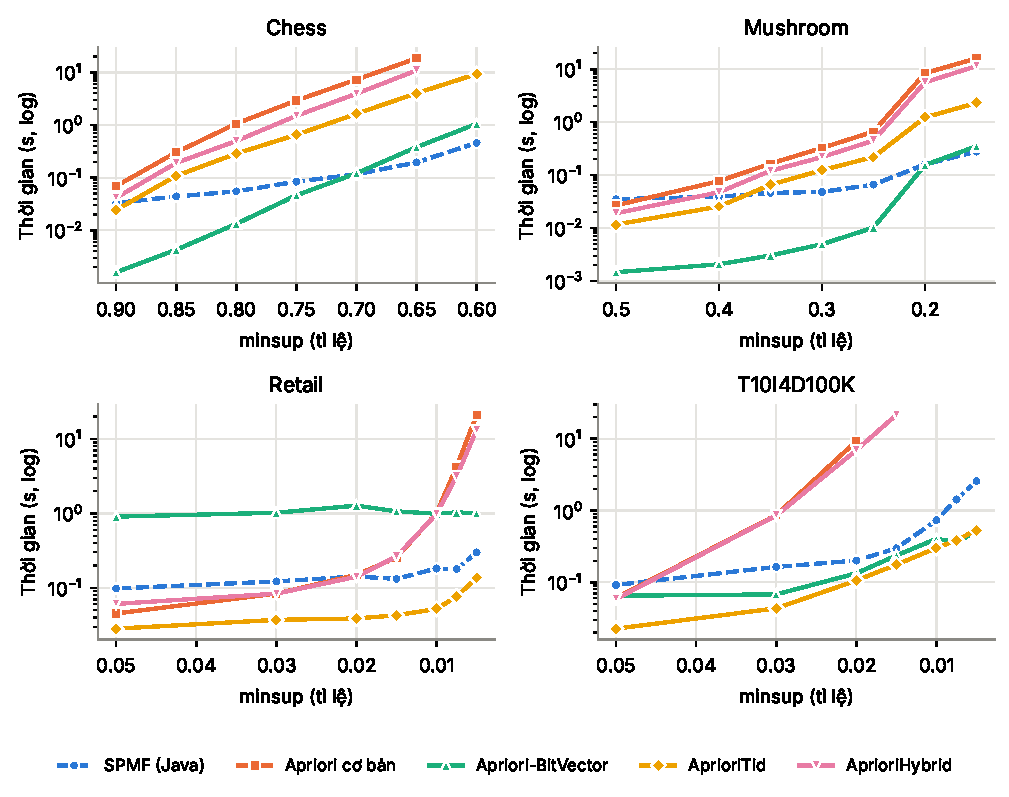
\includegraphics[width=0.82\textwidth]{fig/runtime_vs_minsup.pdf}
\caption{Thời gian chạy theo minsup (giảm dần từ trái sang phải, trục tung log) của 4 biến thể và SPMF. Điểm bị thiếu: lần chạy vượt 30 s.}
\label{fig:runtime}
\end{figure*}

\textbf{Dữ liệu dày (Chess, Mushroom).} Thời gian của mọi biến thể tăng theo hàm mũ khi minsup giảm, song song với số itemset (Hình~\ref{fig:count}). Thứ tự ổn định: BitVector $<$ AprioriTid $<$ AprioriHybrid $<$ cơ bản. Bản cơ bản chậm vì mỗi mức phải kiểm tra $N\cdot|C_k|$ cặp (giao dịch, ứng viên). AprioriTid nhanh hơn bản cơ bản 2,6–7 lần nhưng phải cấp phát tới 11,8 GB (Chess 0,6) vì trên dữ liệu dày mỗi giao dịch chứa rất nhiều ứng viên, đúng như nhận định của bài báo gốc rằng $\bar{C}_k$ có thể lớn hơn CSDL ở các mức đầu. AprioriHybrid nằm giữa: ở dữ liệu dày $|L_k|$ tăng qua nhiều mức nên tiêu chí $|L_k|<|L_{k-1}|$ chỉ thoả muộn, thuật toán đếm bằng Apriori phần lớn thời gian. So với SPMF, bản BitVector nhanh hơn ở minsup cao (ví dụ Chess 0,8: 0,013 s so với 0,055 s, một phần vì SPMF tính cả thời gian đọc file) và chậm hơn khoảng 2 lần ở minsup thấp nhất (Chess 0,6: 1,05 s so với 0,46 s): khi số itemset lớn, chi phí băm khoá \texttt{Vector\{Int\}} và cấp phát một \texttt{BitVector} mới cho mỗi ứng viên chiếm ưu thế.

\textbf{Dữ liệu thưa (Retail, T10I4D100K).} Bức tranh đảo ngược. AprioriTid nhanh nhất trên Retail (0,14 s ở minsup 0,005, nhanh hơn SPMF 2,2 lần) vì $\bar{C}_k$ của dữ liệu thưa rất nhỏ. Trên T10I4D100K, BitVector và AprioriTid nhanh hơn SPMF tới \textbf{5 lần} ở minsup 0,005 (0,51 s so với 2,57 s). Ngược lại, bản cơ bản và Hybrid bùng nổ thời gian ở mức $k=2$: T10I4D100K có hàng trăm item phổ biến (375 item ở minsup 0,01) nên $|C_2|$ cỡ $10^4$–$10^5$, và việc kiểm tra từng ứng viên với từng giao dịch tốn $O(N\,|C_2|)$, vượt 30 s từ minsup 0,015. Đây là chỗ bài báo gốc dùng hash-tree; bản cài đặt của nhóm chưa có cấu trúc này (Mục~\ref{sec:discuss}). Riêng bản BitVector trên Retail giữ quanh 1 s bất kể minsup: thời gian bị chi phối bởi bước dựng bitset ban đầu (xem Mục~\ref{sec:mem}).

\subsection{Số lượng tập phổ biến theo minsup}
Hình~\ref{fig:count} cho thấy số itemset tăng theo hàm mũ khi minsup giảm, nhưng tốc độ rất khác giữa hai loại dữ liệu. Trên Chess, giảm minsup từ 0,9 xuống 0,6 làm số itemset tăng 410 lần (622 $\to$ 254{.}944) và độ dài lớn nhất từ 7 lên 14; trên Mushroom từ 163 lên 99{.}071 (minsup 0,5 $\to$ 0,15). Trên dữ liệu thưa, cùng hệ số giảm minsup chỉ cho vài trăm đến một nghìn itemset, dài tối đa 5 (Retail: 16 $\to$ 580; T10I4D100K: 10 $\to$ 1{.}073). Nguyên nhân: giao dịch dày dài và các item tương quan mạnh, nên khi một itemset dài phổ biến thì toàn bộ $2^k$ tập con của nó cũng phổ biến. Vì vậy minsup ``hợp lý'' phụ thuộc mạnh vào mật độ CSDL: 0,6–0,9 cho dữ liệu dày và 0,5–5\% cho dữ liệu thưa. Thời gian chạy (Hình~\ref{fig:runtime}) bám sát đường cong này, khẳng định chi phí của họ Apriori tỉ lệ với kích thước đầu ra và số ứng viên.

\textbf{Phân bố theo kích thước $k$.} Hình~\ref{fig:levels} vẽ $|L_k|$ theo $k$ từ file thống kê của CLI. Trên dữ liệu dày, $|L_k|$ có dạng ``chuông'': tăng nhanh tới đỉnh ở giữa (Chess 0,8: 2{.}130 tập ở $k=5$; Mushroom 0,2: 10{.}105 tập ở $k=7$) rồi giảm, với tập dài nhất 10 và 15 item. Điều này giải thích hai hành vi đã quan sát: (i) Apriori phải thực hiện nhiều lượt (10–15 mức), mỗi lượt có hàng nghìn ứng viên; (ii) với AprioriHybrid, điều kiện chuyển $|L_k|<|L_{k-1}|$ chỉ thoả sau đỉnh (từ $k\approx6$–8), nên phần lớn công việc vẫn do Apriori đếm. Trên Retail 0,02, $|L_k|$ đạt đỉnh sớm ở $k=2$ (22 tập) rồi giảm ngay — phân bố điển hình của dữ liệu thưa, nơi AprioriTid phát huy tác dụng từ những mức đầu.

\begin{figure}[t]
\centering
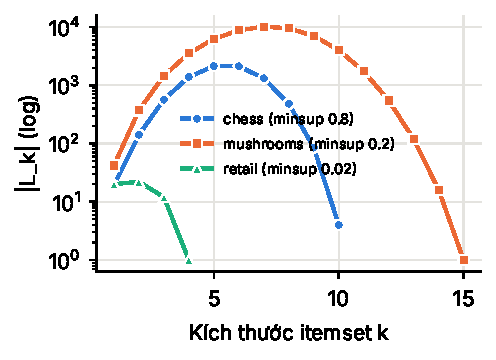
\includegraphics[width=\columnwidth]{fig/levels.pdf}
\caption{Số tập phổ biến $|L_k|$ theo kích thước $k$ (trục tung log).}
\label{fig:levels}
\end{figure}

\begin{figure*}[t]
\centering
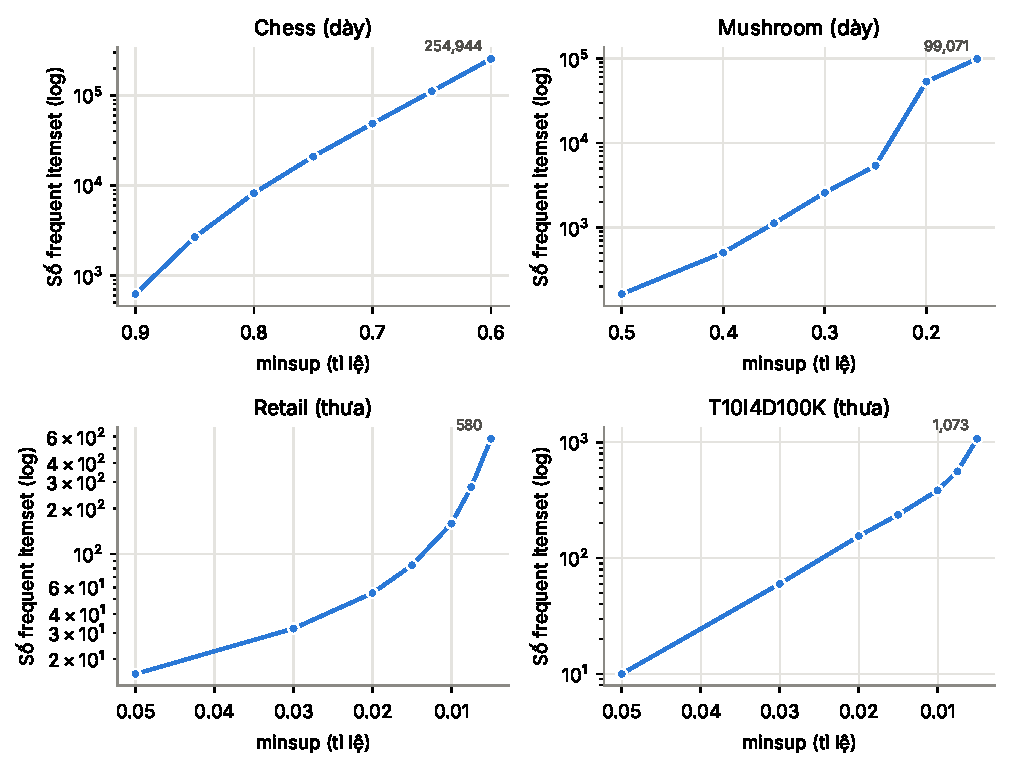
\includegraphics[width=0.7\textwidth]{fig/count_vs_minsup.pdf}
\caption{Số frequent itemset theo minsup (trục tung log). Số trên mỗi đồ thị: số itemset ở minsup thấp nhất.}
\label{fig:count}
\end{figure*}

\subsection{Sử dụng bộ nhớ}\label{sec:mem}
Hình~\ref{fig:mem} báo cáo phần peak RAM \emph{tăng thêm} khi chạy thuật toán (peak RSS sau khi chạy trừ peak RSS sau khi nạp CSDL và runtime Julia — khoảng 230–260 MB nền) tại minsup trung bình của mỗi CSDL; Bảng~\ref{tab:mem} bổ sung tổng bộ nhớ cấp phát. Ở dữ liệu dày, bản cơ bản và BitVector gần như không tăng peak (giá trị 0 nghĩa là đỉnh RSS do nạp dữ liệu vẫn cao hơn), trong khi AprioriTid/Hybrid tăng 90–120 MB vì lưu $\bar{C}_k$. Ở minsup thấp khác biệt rõ hơn: Chess 0,6, peak RSS của AprioriTid là 2,5 GB so với 0,46 GB của BitVector. Ngược lại, trên Retail bản BitVector tăng 250 MB và cấp phát 1,57 GB: hàm \texttt{build\_item\_bitsets} tạo một bitset $N$=88{.}162 bit cho \emph{mỗi} trong 16{.}470 item — kể cả item không phổ biến — và tạo nó qua mảng \texttt{Bool} trung gian (8 lần lớn hơn bitset). Đây là điểm yếu cụ thể của bản tối ưu và là hướng cải tiến đầu tiên.

Hình~\ref{fig:alloc} cho thấy tổng bộ nhớ cấp phát theo minsup. Trên dữ liệu dày, đường của AprioriTid nằm trên các biến thể khác khoảng một bậc độ lớn và tăng cùng tốc độ với số itemset (tới 11,8 GB ở Chess 0,6) vì mỗi giao dịch giữ danh sách $\bar{C}_k(t)$ của hàng nghìn ứng viên; bản cơ bản và BitVector có cấp phát gần như bằng nhau và tỉ lệ với kích thước đầu ra. Trên dữ liệu thưa, thứ tự đảo lại: BitVector cấp phát nhiều nhất và gần như hằng số theo minsup (chi phí cố định dựng bitset), còn AprioriTid ít nhất.

\begin{figure*}[t]
\centering
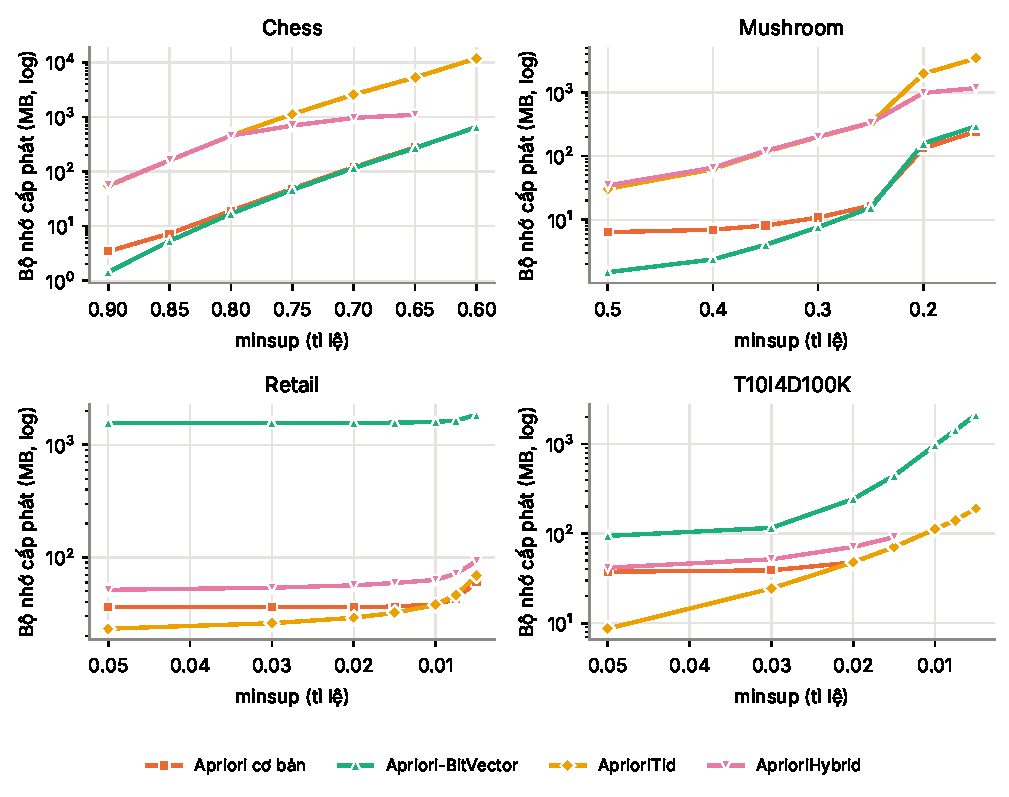
\includegraphics[width=0.82\textwidth]{fig/alloc_vs_minsup.pdf}
\caption{Tổng bộ nhớ cấp phát trong lúc chạy thuật toán (đo bằng \texttt{@timed}, trục tung log) theo minsup.}
\label{fig:alloc}
\end{figure*}

\begin{figure}[t]
\centering
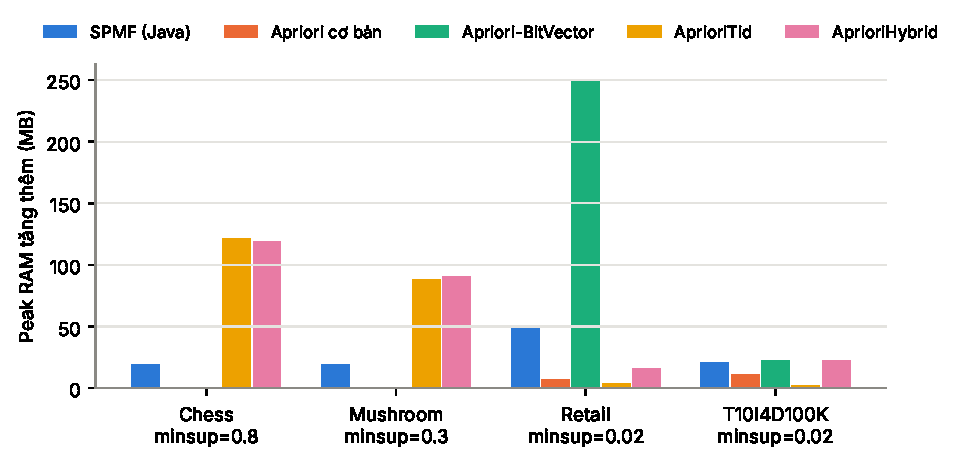
\includegraphics[width=\columnwidth]{fig/memory_peak.pdf}
\caption{Peak RAM tăng thêm khi chạy thuật toán tại minsup trung bình (SPMF: heap JVM do SPMF báo cáo).}
\label{fig:mem}
\end{figure}

\begin{table}[t]
\centering
\caption{Peak RAM tăng thêm / tổng bộ nhớ cấp phát (MB) tại minsup trung bình}
\label{tab:mem}
\footnotesize
\begin{tabular}{@{}lrrrr@{}}
\toprule
Biến thể & Chess 0,8 & Mush. 0,3 & Retail 0,02 & T10 0,02 \\ \midrule
Cơ bản & 0 / 19 & 0 / 11 & 7 / 36 & 11 / 48 \\
BitVector & 0 / 17 & 0 / 8 & 250 / 1566 & 22 / 243 \\
AprioriTid & 121 / 455 & 88 / 199 & 4 / 29 & 2 / 48 \\
AprioriHybrid & 119 / 455 & 90 / 202 & 16 / 57 & 23 / 71 \\
SPMF (heap) & 19 & 19 & 49 & 21 \\
\bottomrule
\end{tabular}
\end{table}

\subsection{Khả năng mở rộng (scalability)}
Nhóm lấy ngẫu nhiên (seed 42, giữ thứ tự gốc) 10\%, 25\%, 50\%, 75\%, 100\% giao dịch của Retail và chạy với minsup tương đối cố định 0,01 (Hình~\ref{fig:scal}). Số itemset gần như không đổi (159–164), nên hình phản ánh thuần chi phí theo $N$. Mọi biến thể tăng \emph{gần tuyến tính}: khi dữ liệu tăng 10 lần, thời gian tăng 10,9 lần (cơ bản), 10,2 lần (Hybrid), 7,0 lần (AprioriTid) và 14,2 lần (BitVector). Điều này khớp với phân tích độ phức tạp: với $|C_k|$ cố định, chi phí mỗi mức tỉ lệ với $N$ (quét CSDL, kích thước $\bar{C}_k$, hay độ dài bitset $N/64$). Bản BitVector tăng nhanh hơn tuyến tính một chút do chi phí dựng bitset $O(|I|\cdot N)$ cho mọi item. AprioriTid nhanh nhất ở mọi kích thước.

\begin{figure}[t]
\centering
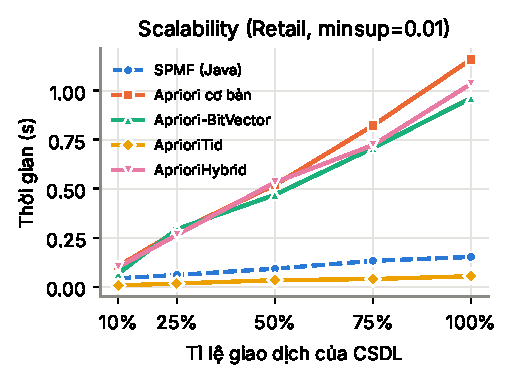
\includegraphics[width=\columnwidth]{fig/scalability.pdf}
\caption{Thời gian theo kích thước CSDL Retail (minsup = 0,01).}
\label{fig:scal}
\end{figure}

\subsection{Ảnh hưởng của độ dài giao dịch trung bình}
Theo phân tích độ phức tạp, chi phí kiểm tra $c\subseteq t$ và số tập con phổ biến của một giao dịch phụ thuộc trực tiếp vào $|t|$. Để kiểm chứng, nhóm sinh 5 CSDL tổng hợp (10{.}000 giao dịch, 1{.}000 item, 20 mẫu ẩn dài 4 item được chèn với xác suất 0,35; seed 42) với độ dài trung bình 5, 10, 15, 20, 25 và chạy ở minsup 0,03 (Hình~\ref{fig:len}). Số itemset giữ quanh 300 tới độ dài 15 rồi tăng vọt (2{.}283 ở độ dài 20; 41{.}470 ở độ dài 25) khi các mẫu ẩn bắt đầu cùng xuất hiện trong một giao dịch và tạo itemset dài tới 8. Thời gian bản cơ bản tăng 91 lần (0,19 $\to$ 17,8 s), Hybrid 136 lần, AprioriTid 83 lần, BitVector chỉ 29 lần (0,009 $\to$ 0,26 s), SPMF 35 lần. Như vậy độ dài giao dịch ảnh hưởng mạnh nhất tới các biến thể duyệt theo giao dịch (cơ bản, Hybrid), trong khi biểu diễn dọc chỉ chịu tác động qua số ứng viên.

\begin{figure}[t]
\centering
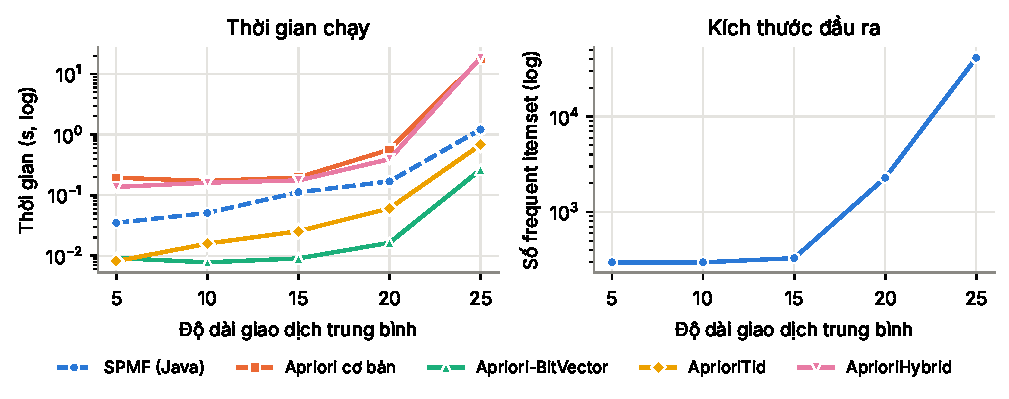
\includegraphics[width=\columnwidth]{fig/length_effect.pdf}
\caption{Ảnh hưởng của độ dài giao dịch trung bình (CSDL tổng hợp, minsup = 0,03).}
\label{fig:len}
\end{figure}

\subsection{Các yếu tố ảnh hưởng đến tính hợp lệ của so sánh}
\textbf{Thời gian.} Thời gian Julia loại trừ đọc file và JIT, trong khi \emph{Total time} của SPMF gồm cả đọc file; ở các minsup cao (thời gian dưới 0,1 s) phần đọc file chiếm phần lớn thời gian SPMF, nên ưu thế của nhóm ở vùng này bị phóng đại. Ở minsup thấp, thời gian thuật toán chiếm ưu thế và so sánh công bằng hơn. Mỗi điểm đo một lần; độ lệch giữa các lần chạy với thời gian dưới 10 ms có thể đáng kể so với giá trị đo.

\textbf{Bộ nhớ.} \texttt{Sys.maxrss} là đỉnh RSS của cả tiến trình (gồm runtime Julia $\approx$230 MB) và có độ phân giải trang bộ nhớ; ``RAM tăng thêm'' bằng 0 chỉ có nghĩa là thuật toán không vượt đỉnh do nạp dữ liệu. SPMF báo heap JVM đã dùng, không gồm bản thân JVM. Vì vậy chỉ nên so sánh bộ nhớ \emph{giữa các biến thể của nhóm}; tổng bộ nhớ cấp phát (Hình~\ref{fig:alloc}) bổ sung một thước đo không phụ thuộc vào thời điểm GC.

\textbf{Giới hạn 30 s.} Các điểm vượt giới hạn bị loại khỏi đồ thị nên đường của bản cơ bản và Hybrid ngắn hơn; điều này không ảnh hưởng tới kết luận định tính về thứ tự giữa các biến thể.

\subsection{Thảo luận: điểm mạnh, điểm yếu và hướng tối ưu}\label{sec:discuss}
\textbf{Điểm mạnh.} (i) Đúng tuyệt đối so với SPMF trên mọi lần chạy; (ii) bản BitVector cạnh tranh với SPMF và nhanh hơn tới 5 lần trên T10I4D100K; (iii) AprioriTid đúng như bài báo — rất hiệu quả trên dữ liệu thưa, nhanh hơn SPMF 2,2 lần trên Retail.

\textbf{Điểm yếu.} (i) Bản cơ bản và Hybrid đếm ứng viên bằng vòng lặp lồng $O(N\,|C_k|)$, khiến mức $k=2$ trên dữ liệu thưa nhiều item trở thành nút cổ chai; (ii) BitVector dựng bitset cho mọi item, tốn 1,5 GB trên Retail; (iii) AprioriTid bùng nổ bộ nhớ trên dữ liệu dày; (iv) khoá \texttt{Vector\{Int\}} trong \texttt{Dict} phải băm cả vector, tốn kém khi có hàng trăm nghìn itemset.

\textbf{Đề xuất tối ưu tiếp theo.}
\begin{enumerate}
\item \emph{Hash-tree hoặc prefix-trie cho bước đếm} (như bài báo gốc): với mỗi giao dịch chỉ duyệt các ứng viên có thể chứa trong nó, thay vì mọi ứng viên; riêng mức 2 dùng ma trận đếm cặp $|L_1|\times|L_1|$ (tam giác) — giảm chi phí từ $O(N\,|C_2|)$ xuống $O(\sum_t|t|^2)$.
\item \emph{Chỉ dựng bitset cho item phổ biến}: đếm support mức 1 trước rồi mới cấp phát bitset bằng \texttt{falses(N)}, loại mảng \texttt{Bool} trung gian; trên Retail chỉ 70 item vượt minsup 0,01 so với 16{.}470 item, dự kiến giảm bộ nhớ và thời gian hơn 100 lần cho bước này.
\item \emph{Diffset (dEclat)} cho dữ liệu dày: lưu $T(P)\setminus T(X)$ thay cho $T(X)$, vốn nhỏ hơn nhiều khi support cao, giảm cả bộ nhớ lẫn thời gian AND.
\item \emph{Mã hoá itemset bằng id nguyên} và lưu support trong mảng, tránh băm \texttt{Vector}; sắp item theo support tăng dần để các nhóm tiền tố nhỏ hơn.
\item \emph{Song song hoá} theo nhóm tiền tố bằng \texttt{Threads.@threads}: các nhóm độc lập nhau ở mỗi mức.
\item \emph{Tiêu chí chuyển của Hybrid} dựa trên ước lượng bộ nhớ như bài báo, thay cho điều kiện $|L_k|<|L_{k-1}|$ — để chuyển sớm sang AprioriTid trên dữ liệu thưa.
\end{enumerate}

%======================================================================
\section{Chương 3: Ứng dụng thực tế}\label{sec:app}
Cả hai ứng dụng dùng chính cài đặt của nhóm (bản Hybrid); mã chuyển đổi dữ liệu và toàn bộ kết quả được tái thực hiện trong notebook Colab.

\subsection{Ứng dụng 1: Phân tích giỏ hàng trên Groceries}
\textbf{Dữ liệu.} Groceries~\cite{hahsler2006} gồm 9{.}835 hoá đơn trong 30 ngày của một cửa hàng tạp hoá, 169 nhóm hàng có tên (ví dụ \textit{whole milk}, \textit{root vegetables}). Nhóm chọn Groceries thay cho Retail vì Retail chỉ có mã số item, không cho phép diễn giải ý nghĩa kinh doanh.

\textbf{Biến đổi thành giao dịch.} Mỗi hoá đơn là một giao dịch; mỗi nhóm hàng được mã hoá thành số nguyên theo thứ tự chữ cái (bảng ánh xạ lưu riêng để giải mã); mặt hàng lặp trong một hoá đơn chỉ tính một lần. CSDL thu được thưa (độ dài trung bình 4,41), vùng Apriori làm việc hiệu quả.

\textbf{Thiết lập.} minsup = 1\% ($\sigma$ = 99 hoá đơn) và minconf = 30\%. Thu được 333 tập phổ biến và \textbf{125 luật}. Luật được sinh bằng \texttt{generate\_rules}: với mỗi tập phổ biến $Z$, duyệt mọi cách chia $Z=X\cup Y$ bằng bitmask; nhờ tính chất Apriori, $\sup(X)$ và $\sup(Y)$ tra trực tiếp từ kết quả mà không quét lại CSDL. Mặt hàng phổ biến nhất là whole milk (25,6\% hoá đơn), other vegetables (19,3\%) và rolls/buns (18,4\%).

\begin{table}[t]
\centering
\caption{Top-10 luật theo lift trên Groceries (minsup 1\%, minconf 30\%)}
\label{tab:rules}
\scriptsize
\setlength{\tabcolsep}{3pt}
\begin{tabular}{@{}r>{\raggedright\arraybackslash}p{2.45cm}>{\raggedright\arraybackslash}p{1.5cm}rrr@{}}
\toprule
\# & $X$ & $Y$ & supp & conf & lift \\ \midrule
1 & citrus fruit, other veg. & root veg. & 0,010 & 0,359 & 3,30 \\
2 & other veg., tropical fruit & root veg. & 0,012 & 0,343 & 3,14 \\
3 & beef & root veg. & 0,017 & 0,331 & 3,04 \\
4 & citrus fruit, root veg. & other veg. & 0,010 & 0,586 & 3,03 \\
5 & root veg., tropical fruit & other veg. & 0,012 & 0,585 & 3,02 \\
6 & other veg., whole milk & root veg. & 0,023 & 0,310 & 2,84 \\
7 & curd, whole milk & yogurt & 0,010 & 0,385 & 2,76 \\
8 & rolls/buns, root veg. & other veg. & 0,012 & 0,502 & 2,59 \\
9 & root veg., yogurt & other veg. & 0,013 & 0,500 & 2,58 \\
10 & tropical fruit, whole milk & yogurt & 0,015 & 0,358 & 2,57 \\
\bottomrule
\end{tabular}
\end{table}

\textbf{Diễn giải kinh doanh.} Bảng~\ref{tab:rules} và Hình~\ref{fig:rules} cho thấy:
\begin{itemize}
\item \emph{Rau củ là vế phải của 8/10 luật đầu.} Khách đã mua hai nhóm rau củ/trái cây có xác suất mua nhóm thứ ba cao gấp khoảng 3 lần mức trung bình (lift $\approx$ 3), phản ánh hành vi ``đi chợ nấu ăn cả tuần''. Gợi ý: bố trí quầy rau củ và trái cây liền kề, bán combo ``giỏ rau tuần'', khuyến mãi chéo giữa các nhóm đồ tươi.
\item \emph{beef $\Rightarrow$ root vegetables} (conf 33\%, lift 3,04): thịt bò thường được mua cùng rau củ cho món hầm/nướng. Gợi ý: trưng bày rau củ cạnh quầy thịt, in công thức món ăn kèm danh sách nguyên liệu.
\item \emph{Cụm sữa:} \{curd, whole milk\} $\Rightarrow$ yogurt và \{tropical fruit, whole milk\} $\Rightarrow$ yogurt (lift 2,6–2,8) gợi ý nhu cầu bữa sáng; có thể bán bundle sữa chua + trái cây.
\item \emph{Vì sao xếp theo lift?} whole milk và other vegetables có support riêng rất cao nên xuất hiện ở vế phải của nhiều luật có confidence cao nhưng lift thấp — đó là các luật ``hiển nhiên''. Lift chuẩn hoá theo độ phổ biến của $Y$ nên làm nổi bật các liên kết thực sự.
\end{itemize}
\textbf{Cấu trúc tập luật và độ nhạy theo ngưỡng.} Trong 125 luật, 69 luật có vế trái 1 item và 56 luật có vế trái 2 item (không có tập phổ biến nào dài hơn 3 ở minsup 1\%). Vế phải tập trung mạnh: 66 luật dẫn tới \textit{whole milk} và 44 luật dẫn tới \textit{other vegetables}, xác nhận vai trò ``mặt hàng neo'' của hai nhóm này. Bảng~\ref{tab:sens} cho thấy số luật rất nhạy với ngưỡng: hạ minsup từ 2\% xuống 0,5\% làm số tập phổ biến tăng 8 lần và số luật tăng 13 lần, đồng thời xuất hiện các luật có lift cao hơn (tới 4,72, ví dụ \{pip fruit, root vegetables\} $\Rightarrow$ \{other vegetables, whole milk\}) nhưng support chỉ khoảng 0,5\%. Nâng minconf lên 50\% loại phần lớn luật. Mức (1\%, 30\%) được chọn vì cân bằng giữa số luật đủ để phân tích và độ tin cậy thống kê (mỗi luật dựa trên ít nhất 99 hoá đơn).

\begin{table}[t]
\centering
\caption{Độ nhạy theo ngưỡng trên Groceries (chạy bằng cài đặt của nhóm)}
\label{tab:sens}
\footnotesize
\begin{tabular}{@{}rrrrr@{}}
\toprule
minsup & minconf & \#tập phổ biến & \#luật & lift lớn nhất \\ \midrule
2\% & 30\% & 122 & 37 & 2,84 \\
2\% & 50\% & 122 & 1 & 2,01 \\
1\% & 30\% & 333 & 125 & 3,30 \\
1\% & 50\% & 333 & 15 & 3,03 \\
0,5\% & 30\% & 1{.}001 & 487 & 4,72 \\
0,5\% & 50\% & 1{.}001 & 120 & 3,69 \\
\bottomrule
\end{tabular}
\end{table}

\textbf{Từ luật đến hành động.} Tập luật có thể đưa vào vận hành theo ba cách. (i) \emph{Gợi ý tại quầy thanh toán hoặc trên ứng dụng}: với giỏ hàng hiện tại $B$, chọn các luật $X\Rightarrow Y$ có $X\subseteq B$ và $Y\not\subseteq B$, xếp theo lift rồi confidence, gợi ý $Y$ của luật đầu tiên — ví dụ giỏ có beef nhưng chưa có rau củ sẽ được gợi ý root vegetables. (ii) \emph{Bố trí cửa hàng}: các cặp lift cao (rau củ – trái cây, sữa – sữa chua) nên đặt gần nhau hoặc trên cùng lối đi, còn các mặt hàng neo như whole milk có thể đặt cuối cửa hàng để kéo khách đi qua nhiều quầy. (iii) \emph{Thiết kế khuyến mãi}: chỉ nên giảm giá vế trái của luật có lift cao, vì doanh thu kéo theo từ vế phải mới thực sự tăng thêm; khuyến mãi whole milk ít hiệu quả vì khách đã mua nó với xác suất cao. Cả ba cách đều cần cập nhật luật định kỳ (ví dụ hàng tháng) vì hành vi mua sắm thay đổi theo mùa.

\textbf{Giới hạn.} Lift đo đồng xuất hiện chứ không phải nhân quả; dữ liệu 30 ngày của một cửa hàng; các luật top có support chỉ 1–2\% nên cần kiểm chứng (ví dụ A/B test) trước khi triển khai khuyến mãi.

\begin{figure}[t]
\centering
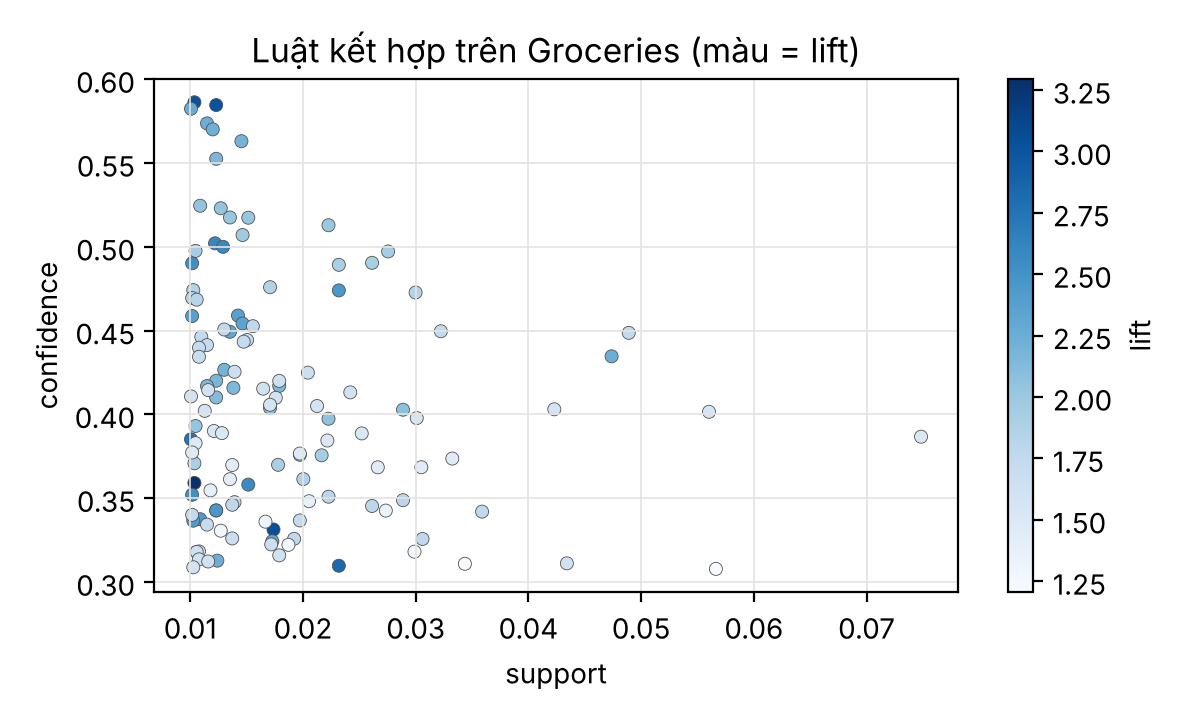
\includegraphics[width=\columnwidth]{fig/rules_scatter.png}
\caption{125 luật trên Groceries theo support và confidence; màu thể hiện lift.}
\label{fig:rules}
\end{figure}

\subsection{Ứng dụng 2: Phân tích dữ liệu sinh học trên genome SARS-CoV-2}
\textbf{Dữ liệu.} Genome SARS-CoV-2 GenBank MT745584 (29{.}860 nucleotide, GC = 38,0\%), định dạng FASTA.

\textbf{Biến đổi thành giao dịch.} Genome được cắt bằng cửa sổ trượt dài $W=100$ nt, bước $S=50$ nt (chồng lấn 50\%), mỗi cửa sổ là một giao dịch (596 giao dịch). Item là các \emph{3-mer} (chuỗi con 3 nucleotide) xuất hiện trong cửa sổ, mã hoá thành 64 số nguyên. Lựa chọn $k=3$ xuất phát từ thử nghiệm: với $k=6$ (4{.}096 item, mỗi cửa sổ chỉ chứa tối đa 95), CSDL quá thưa — ở minsup 10\% chỉ có 12 itemset, toàn bộ kích thước 1, không có tổ hợp nào để phân tích. Với $k=3$, mỗi cửa sổ chứa trung bình 45,3/64 item, tạo một CSDL \emph{dày} mà Apriori (đặc biệt bản BitVector/Hybrid) xử lý tốt, và các tập phổ biến phản ánh \emph{thành phần nucleotide} của từng vùng genome.

\textbf{Chọn tham số biến đổi.} Bảng~\ref{tab:grid} so sánh các cấu hình thử nghiệm (đều chạy bằng cài đặt của nhóm trong notebook). Với $k$ lớn, CSDL thưa và chỉ thu được tập 1 phần tử; với $k=4$ và cửa sổ 150 nt mới xuất hiện 3 tập đôi. Cấu hình $k=3$, $W=100$, $S=50$ cho cấu trúc phong phú nhất (106 tập đôi, 51 tập ba) mà vẫn đủ nhỏ để diễn giải.

\begin{table}[t]
\centering
\caption{Ảnh hưởng của cách biến đổi genome thành giao dịch}
\label{tab:grid}
\footnotesize
\setlength{\tabcolsep}{4pt}
\begin{tabular}{@{}rrrrrrl@{}}
\toprule
$k$ & $W$ & $S$ & minsup & \#gd & Độ dài TB & \#itemset (theo kích thước) \\ \midrule
6 & 100 & 95 & 0,1 & 314 & 93,0 & 12 (12 đơn) \\
4 & 100 & 50 & 0,5 & 596 & 75,8 & 23 (23 đơn) \\
4 & 150 & 75 & 0,6 & 397 & 101,9 & 50 (47 đơn, 3 đôi) \\
3 & 100 & 50 & 0,8 & 596 & 45,3 & 186 (29/106/51) \\
\bottomrule
\end{tabular}
\end{table}

\textbf{Kết quả.} Ở minsup 0,8 thu được 186 tập phổ biến (29 đơn, 106 đôi, 51 bộ ba), ở minsup 0,7 là 2{.}527 tập dài tới 5 item. Các tổ hợp phổ biến nhất đều giàu T (U trên RNA), ví dụ \{GTT, TTA, TTG\} có mặt ở 83,1\% đoạn và \{CTT, TTA, TTG\} ở 82,6\%. Chạy thêm với \texttt{--maxlen 1} để lấy support của cả 64 3-mer (Hình~\ref{fig:kmer}). Bảng~\ref{tab:kmer} đối chiếu các tổ hợp phổ biến nhất với các 3-mer hiếm nhất.

\begin{table}[t]
\centering
\caption{Trái: 6 tổ hợp 3 phần tử phổ biến nhất (minsup 0,8); phải: 8 3-mer hiếm nhất (support = tỉ lệ trong 596 đoạn)}
\label{tab:kmer}
\footnotesize
\begin{tabular}{@{}lr@{\hspace{1.2em}}lr@{}}
\toprule
Tổ hợp 3-mer & supp & 3-mer & supp \\ \midrule
GTT + TTA + TTG & 0,831 & CCG & 0,215 \\
CTT + TTA + TTG & 0,826 & CGG & 0,220 \\
ACA + TTA + TTG & 0,826 & GCG & 0,238 \\
TTA + TTG + TTT & 0,820 & CGA & 0,257 \\
TGT + TTA + TTG & 0,820 & CGC & 0,267 \\
AAT + TTA + TTG & 0,819 & TCG & 0,285 \\
 & & CCC & 0,292 \\
 & & GGG & 0,342 \\
\bottomrule
\end{tabular}
\end{table}

\begin{figure*}[t]
\centering
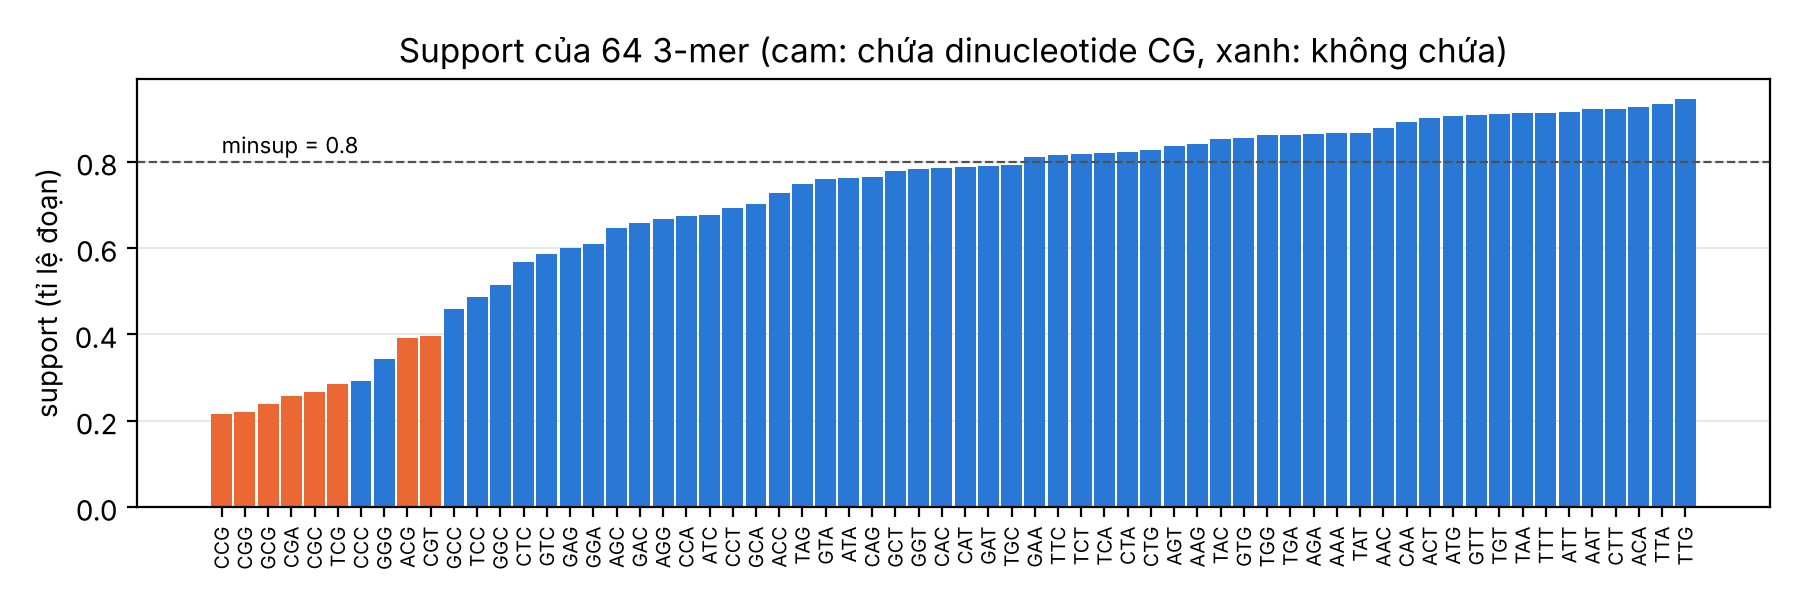
\includegraphics[width=0.9\textwidth]{fig/kmer_support.png}
\caption{Support của 64 3-mer trên genome SARS-CoV-2 (tỉ lệ cửa sổ chứa 3-mer). Cam: 3-mer chứa dinucleotide CG; đường nét đứt: minsup 0,8.}
\label{fig:kmer}
\end{figure*}

\textbf{Ý nghĩa sinh học.}
\begin{itemize}
\item \emph{Ức chế CpG.} Không tập phổ biến nào (ở cả minsup 0,8 và 0,7) chứa 3-mer mang dinucleotide CG; trong Hình~\ref{fig:kmer}, \textbf{cả 8 3-mer chứa CG đều nằm trong nhóm 10 3-mer hiếm nhất} (support 21–40\%, trong khi phần lớn 3-mer khác trên 60\%). Tỉ lệ quan sát/kỳ vọng của CG trên genome là 0,41, tức CG bị thiếu hụt mạnh ngay cả khi đã tính đến GC thấp. Kết quả này khớp với phát hiện ``thiếu hụt CpG cực độ'' ở SARS-CoV-2~\cite{xia2020}; một giả thuyết được ủng hộ rộng rãi là áp lực chọn lọc từ protein kháng virus ZAP — vốn nhận diện RNA giàu CpG~\cite{takata2017} — khiến virus giảm CpG để né miễn dịch bẩm sinh của vật chủ.
\item \emph{Thiên lệch giàu A/U.} Các tổ hợp phổ biến chủ yếu gồm 3-mer giàu T/A. Đáng chú ý TTA, TTG, CTT đều là codon mã hoá Leucine; tuy nhiên cửa sổ trượt không theo khung đọc nên đây chỉ là gợi ý cần kiểm chứng trên vùng mã hoá.
\item \emph{Khả năng ứng dụng.} Tập k-mer phổ biến/bị thiếu là ``chữ ký thành phần'' có thể dùng làm đặc trưng phân loại virus theo họ hoặc vật chủ, phát hiện đoạn bất thường (một cửa sổ giàu CpG bất thường có thể là vùng tái tổ hợp hoặc trình tự ngoại lai), và hỗ trợ thiết kế virus giảm độc lực bằng cách tăng CpG có chủ đích.
\end{itemize}
\textbf{Giới hạn.} Phân tích một genome duy nhất nên các tập phổ biến phản ánh thành phần hơn là motif chức năng. Hướng mở rộng: coi mỗi chủng virus là một giao dịch các đột biến để tìm các tổ hợp đột biến cùng xuất hiện giữa các biến thể.

%======================================================================
\section{Kết luận}
Nhóm đã cài đặt lại từ bài báo gốc ba thuật toán Apriori, AprioriTid, AprioriHybrid và một biến thể tối ưu dùng tidset \texttt{BitVector} bằng Julia, đạt kết quả khớp 100\% với SPMF trên 103/103 lần so sánh và 5 CSDL kiểm thử. Thực nghiệm xác nhận các nhận định của bài báo: AprioriTid vượt trội trên dữ liệu thưa nhưng tốn bộ nhớ trên dữ liệu dày, chi phí mọi biến thể tăng theo hàm mũ khi giảm minsup và theo độ dài giao dịch, và tuyến tính theo số giao dịch. Biến thể BitVector nhanh hơn bản cơ bản 18–80 lần trên dữ liệu dày và nhanh hơn SPMF tới 5 lần trên T10I4D100K, nhưng cần cải tiến bước dựng bitset trên dữ liệu nhiều item. Hai ứng dụng cho thấy FIM vừa tìm được các quy luật mua sắm có thể hành động trên Groceries, vừa tái phát hiện một đặc trưng sinh học đã biết (ức chế CpG) trên genome SARS-CoV-2 mà không cần tri thức chuyên ngành đưa vào trước.

\textbf{Bài học rút ra.} (i) Không có biến thể nào tốt nhất trên mọi dữ liệu: biểu diễn dọc thắng trên dữ liệu dày, AprioriTid thắng trên dữ liệu thưa — đúng tinh thần ``hybrid'' của bài báo gốc, nhưng tiêu chí chuyển cần được thiết kế cẩn thận. (ii) Kiểm thử đối chiếu với một cài đặt tham chiếu và với brute force trên dữ liệu ngẫu nhiên phát hiện lỗi sớm hơn nhiều so với kiểm tra thủ công. (iii) Trong ứng dụng, bước biến đổi dữ liệu thành giao dịch quyết định chất lượng kết quả nhiều hơn bản thân thuật toán: cùng một genome, $k=6$ cho kết quả gần như vô nghĩa còn $k=3$ làm lộ ra hiện tượng sinh học rõ rệt.

\textbf{Hướng phát triển.} Ngoài các tối ưu đã nêu ở Mục~\ref{sec:discuss} (hash-tree/ma trận đếm cặp, chỉ dựng bitset cho item phổ biến, diffset, song song hoá), nhóm dự định: cài đặt FP-Growth bằng cùng khung kiểm thử để so sánh với họ Apriori; mở rộng Ứng dụng 2 sang nhiều chủng SARS-CoV-2 (mỗi chủng một giao dịch gồm các đột biến) để tìm tổ hợp đột biến đồng xuất hiện; và áp dụng tập luật Groceries vào bài toán gợi ý sản phẩm, đánh giá bằng độ chính xác dự đoán món hàng tiếp theo trên tập kiểm tra.

%======================================================================
\begin{thebibliography}{99}
\footnotesize
\bibitem{agrawal1994} R. Agrawal and R. Srikant, ``Fast algorithms for mining association rules,'' in \textit{Proc. 20th Int. Conf. Very Large Data Bases (VLDB)}, Santiago, Chile, 1994, pp. 487--499.
\bibitem{agrawal1993} R. Agrawal, T. Imieliński, and A. Swami, ``Mining association rules between sets of items in large databases,'' in \textit{Proc. ACM SIGMOD}, 1993, pp. 207--216.
\bibitem{spmf2016} P. Fournier-Viger \textit{et al.}, ``The SPMF open-source data mining library version 2,'' in \textit{Proc. ECML PKDD}, 2016, pp. 36--40.
\bibitem{zaki2000} M. J. Zaki, ``Scalable algorithms for association mining,'' \textit{IEEE Trans. Knowl. Data Eng.}, vol. 12, no. 3, pp. 372--390, 2000.
\bibitem{han2000} J. Han, J. Pei, and Y. Yin, ``Mining frequent patterns without candidate generation,'' in \textit{Proc. ACM SIGMOD}, 2000, pp. 1--12.
\bibitem{brin1997} S. Brin, R. Motwani, J. D. Ullman, and S. Tsur, ``Dynamic itemset counting and implication rules for market basket data,'' in \textit{Proc. ACM SIGMOD}, 1997, pp. 255--264.
\bibitem{goethals2003} B. Goethals and M. J. Zaki, ``Advances in frequent itemset mining implementations: Introduction to FIMI03,'' in \textit{Proc. IEEE ICDM Workshop on Frequent Itemset Mining Implementations}, 2003.
\bibitem{zheng2001} Z. Zheng, R. Kohavi, and L. Mason, ``Real world performance of association rule algorithms,'' in \textit{Proc. ACM SIGKDD}, 2001, pp. 401--406.
\bibitem{brijs1999} T. Brijs, G. Swinnen, K. Vanhoof, and G. Wets, ``Using association rules for product assortment decisions: A case study,'' in \textit{Proc. ACM SIGKDD}, 1999, pp. 254--260.
\bibitem{hahsler2006} M. Hahsler, K. Hornik, and T. Reutterer, ``Implications of probabilistic data modeling for mining association rules,'' in \textit{From Data and Information Analysis to Knowledge Engineering}, Springer, 2006, pp. 598--605.
\bibitem{xia2020} X. Xia, ``Extreme genomic CpG deficiency in SARS-CoV-2 and evasion of host antiviral defense,'' \textit{Mol. Biol. Evol.}, vol. 37, no. 9, pp. 2699--2705, 2020.
\bibitem{takata2017} M. A. Takata \textit{et al.}, ``CG dinucleotide suppression enables antiviral defence targeting non-self RNA,'' \textit{Nature}, vol. 550, pp. 124--127, 2017.
\bibitem{bezanson2017} J. Bezanson, A. Edelman, S. Karpinski, and V. B. Shah, ``Julia: A fresh approach to numerical computing,'' \textit{SIAM Review}, vol. 59, no. 1, pp. 65--98, 2017.
\end{thebibliography}

%======================================================================
\onecolumn
\appendix
\section*{Phụ lục: Thời gian chạy chi tiết (giây)}
TO: vượt giới hạn 30 s hoặc bị bỏ qua vì minsup cao hơn đã vượt giới hạn. Thời gian Julia không gồm đọc file và biên dịch JIT; thời gian SPMF gồm cả đọc file.
\begin{center}
\small
\begin{tabular}{ll rrrrrr}
\toprule
CSDL & minsup & \#itemset & SPMF & Basic & BitVector & Tid & Hybrid \\
\midrule
T10I4D100K & 0.05 & 10 & 0.09 & 0.06 & 0.07 & 0.02 & 0.06 \\
T10I4D100K & 0.03 & 60 & 0.16 & 0.86 & 0.07 & 0.04 & 0.85 \\
T10I4D100K & 0.02 & 155 & 0.20 & 9.27 & 0.13 & 0.11 & 6.92 \\
T10I4D100K & 0.015 & 237 & 0.30 & TO & 0.24 & 0.18 & 21.48 \\
T10I4D100K & 0.01 & 385 & 0.73 & TO & 0.40 & 0.30 & TO \\
T10I4D100K & 0.0075 & 561 & 1.42 & TO & 0.36 & 0.39 & TO \\
T10I4D100K & 0.005 & 1{,}073 & 2.56 & TO & 0.51 & 0.53 & TO \\
Chess & 0.9 & 622 & 0.03 & 0.07 & 0.00 & 0.02 & 0.04 \\
Chess & 0.85 & 2{,}669 & 0.04 & 0.30 & 0.00 & 0.11 & 0.19 \\
Chess & 0.8 & 8{,}227 & 0.06 & 1.06 & 0.01 & 0.29 & 0.50 \\
Chess & 0.75 & 20{,}993 & 0.08 & 2.93 & 0.05 & 0.65 & 1.50 \\
Chess & 0.7 & 48{,}731 & 0.12 & 7.31 & 0.12 & 1.64 & 3.94 \\
Chess & 0.65 & 111{,}239 & 0.20 & 18.50 & 0.38 & 4.02 & 10.93 \\
Chess & 0.6 & 254{,}944 & 0.46 & TO & 1.05 & 9.33 & TO \\
Mushroom & 0.5 & 163 & 0.04 & 0.03 & 0.00 & 0.01 & 0.02 \\
Mushroom & 0.4 & 505 & 0.04 & 0.08 & 0.00 & 0.03 & 0.05 \\
Mushroom & 0.35 & 1{,}121 & 0.05 & 0.16 & 0.00 & 0.07 & 0.12 \\
Mushroom & 0.3 & 2{,}587 & 0.05 & 0.33 & 0.00 & 0.12 & 0.22 \\
Mushroom & 0.25 & 5{,}393 & 0.07 & 0.66 & 0.01 & 0.22 & 0.45 \\
Mushroom & 0.2 & 53{,}337 & 0.16 & 8.42 & 0.15 & 1.23 & 5.66 \\
Mushroom & 0.15 & 99{,}071 & 0.28 & 16.04 & 0.35 & 2.31 & 11.44 \\
Retail & 0.05 & 16 & 0.10 & 0.05 & 0.91 & 0.03 & 0.06 \\
Retail & 0.03 & 32 & 0.12 & 0.08 & 1.02 & 0.04 & 0.08 \\
Retail & 0.02 & 55 & 0.14 & 0.15 & 1.27 & 0.04 & 0.14 \\
Retail & 0.015 & 84 & 0.13 & 0.25 & 1.06 & 0.04 & 0.26 \\
Retail & 0.01 & 159 & 0.18 & 1.01 & 0.99 & 0.05 & 0.99 \\
Retail & 0.0075 & 277 & 0.18 & 4.24 & 1.03 & 0.08 & 3.13 \\
Retail & 0.005 & 580 & 0.30 & 21.11 & 1.01 & 0.14 & 13.21 \\
\bottomrule
\end{tabular}
\end{center}
\end{document}
